\section{Theoretische Vorbereitung}
    %http://muenchuwe.com/nonhtml/papers/fest-25.pdf
    \subsection{Kristallstrukturen}
        Kristalline Festkörper lassen sich durch Kristallstrukturen beschreiben. Eine Kristallstruktur besteht
        dabei in der Regel aus einer endlichen Aneinanderreihung der sogenannten Elementarzelle. Die Elementarzelle ist
        jene Zelle, bestehend aus einer Gruppe von Atomen an ihren Gitterpunkten, die durch lückenloses und translationssymetrisches Aneinanderfügen das Gitter erzeugt.
        Diese lässt sich noch einmal aufteilen in die sogenannte Basis. Diese ist die kleinste Gruppe Atome, die
        sich in dem fraglichen Gitter wiederholt. Elementarzelle und Basiszelle können in manchen Fällen äquivalent sein.
    \subsection{Gitterfehler}
        Innerhalb der Gitter kann es zu Abweichungen von der perfekten kristallinen Struktur kommen. Diese Gitterfehler lassen
        sich in verschiedene Gruppen aufteilen.
        \subsubsection*{Nulldimensionale Fehler}
            Punktdefekte beschreiben die Veränderung einzelner Atome im Gitter. Dabei kann es vorkommen, dass 
            einzelne Gitterpunkte nicht besetzt sind und somit eine \textbf{Leerstelle} bilden.
            Alternativ kann es dazu kommen, dass eine Gitterposition von einem andersartigen Atom besetzt wird.
            Derartige Fehlstellen werden auch als \textbf{Substitutionsatome} bezeichnet.
            Zuletzt kann es zu Besetzungen von Gitterplätzen kommen, die im regulären Gitter gar nicht vorhanden sind.
            Solche Besetzungen bezeichnet man als \textbf{Zwischengitteratome}.\\
            Punktfehler lassen sich noch weiter differenzieren, da Punktdefekte für diesen Versuch jedoch keine besondere
            Rolle spielen, möchten wir an dieser Stelle auf Fachliteratur verweisen.
        \subsubsection*{Eindimensionale Fehler}
            Linienfehler oder auch \textbf{Versetzungen} sind hier von besonderem Interesse. Linienfehler haben 
            großen Einfluss auf die mechanischen Eigenschaften eines Festkörpers, was
            als Nachweismethode solcher Fehler im Kristall genutzt werden kann. Eine Versetzung ist im Allgemeinen eine Störung des periodischen Gitters, 
            die sich, anders als Punktdefekte, entlang einer Linie im Kristall fortsetzt. Sie entstehen durch Krafteinwirkungen auf das Gitter,
            durch Eigenspannung, beim Wachstum oder durch äußere Kräfte bei plastischer Deformation.\\
            Bei Versetzungen wird zwischen Stufenversetzungen und Schraubenversetzungen unterschieden.
            Sie werden durch den Burgers - Vektor charakterisiert, der im nächsten Abschnitt näher erklärt wird.
            Bei Stufenversetzung stehen der Burgers - Vektor und die Versetzungslinie senkrecht zueinander.
            \begin{figure}[H]
                \centering
                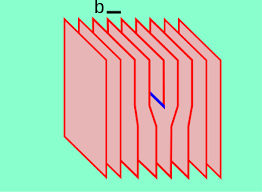
\includegraphics[width=0.5\textwidth]{Images/Stufenversetzung.png}
                \caption{Schematische Darstellung einer Stufenversetzung [5]}
            \end{figure}
            Bei Schraubenversetzungen hingegen stehen Burgers - Vektor und Gleitvektor parallel zueinander.
            \begin{figure}[H]
                \centering
                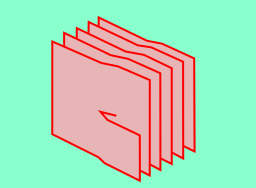
\includegraphics[width=0.5\textwidth]{Images/Schraubenversetzung.png}
                \caption{Schematische Darstellung einer Schraubenversetzung [5]}
            \end{figure}
        \subsubsection*{Zweidimensionale Fehler}
            Eine weiter Gruppe Gitterfehler sind die \textbf{Flächenfehler}. Den wohl simpelsten Flächenfehler
            stellt die Oberfläche eines Kristalls dar, da dort eine Unterbrechung der Periodizität und Translationssymetrie vorliegt.
            Ein anderer Flächenfehler ist die sogenannte \textbf{Korngrenze}. An Korngrenzen kommen zwei 
            Bereiche des Kristallgitters mit verschiedener räumlicher Orientierung zueinander zusammen. Diese Grenzen lassen sich anhand ihrer Winkel
            anschließend noch in Kleinwinkelkorngrenzen und Großwinkelkorngrenzen unterteilen.
            \begin{figure}[H]
                \centering
                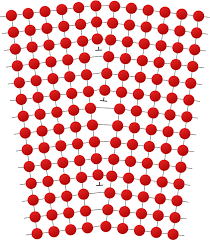
\includegraphics[width=0.5\textwidth]{Images/Kleinwinkelkorngrenze.png}
                \caption{Schematische Darstellung einer Kleinwinkelkorngrenze [4]}
            \end{figure}
            Sogenannte \textbf{Stapelfehler} bezeichnen Fehler in der Stapelreihenfolge in einem Kristallgitter. Solche Fehler in der Periodizität
            können zu Bildungen von Kleinwinkelkorngrenzen führen.
            Weitere zweidimensionale Fehler sind die Antiphasengrenze und die Zwillingsgrenze sowie Domänenwände, diese tragen jedoch nicht
            zu diesem Versuch bei und werden daher hier nicht näher beschrieben.
        \subsubsection*{Dreidimensionale Fehler}
            Die letzte Gruppe ist die Gruppe der dreidimensionalen Fehler, oder auch Volumenfehler. Sie bezeichnen Einbindungen vollständig verschiedener Stoffe innerhalb der ursprünglichen
            Kristallstruktur. So bezeichnen \textbf{Poren} Hohlräume im Kristall, die mit Gas oder Flüssigkeit gefüllt sind, wohingegen
            \textbf{Einschlüsse} derart in den Kristall integrierte Festkörper beschreiben.
            Diese Fehler sind in der Regel von makroskopischer Größenordnung, führen jedoch an ihren Grenzen zum ursprünglichen Kristallgitter
            zu einer Reihe niederdimensionaler Gitterfehler.

    \subsection{Lithiumfluorid}
	\begin{figure}[H]
            \centering
            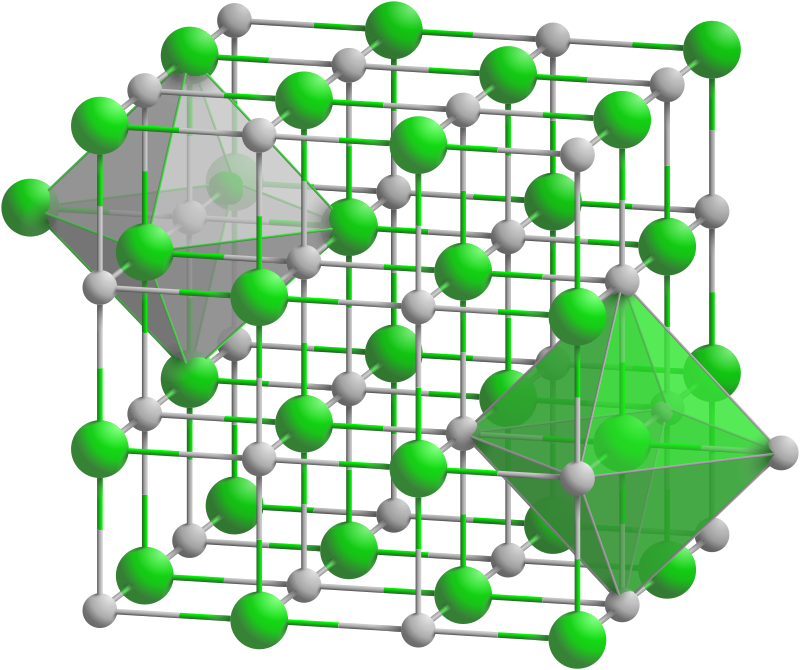
\includegraphics[width=0.5\textwidth]{Images/LiF.PNG}
            \caption{LiF - Kristallstruktur. [6]}
            \label{FigLiF}
        \end{figure}
	LiF gehört zur Stoffklasse der Alkalihalogenide und ist ein Salz, das in der NaCl - Struktur kristallisiert. Die NaCl - Struktur wird beschrieben durch ein fcc - Gitter und eine
	zweiatomige Basis. Es handelt sich also um ein kubisches Gitter, dessen Gitterpunkte
	abwechselnd von den zwei unterschiedlichen Atomsorten besetzt werden, sodass jedes Atom der einen Sorte stets nur Atome der jeweils anderen Sorte als nächste Nachbarn hat.
	Die Atome jeweils einer Sorte besetzen somit ein \textbf{kubisch flächenzentriertes Gitter} (kurz FCC), wie in Abb. \ref{FigLiF} zu erkennen ist. 


    \subsection{Burgers Vektor}

	\begin{figure}[H]
            \centering
            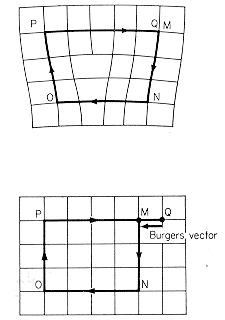
\includegraphics[width=0.5\textwidth]{Images/Burger.PNG}
            \caption{Konstruktion des Burgers - Vektors. [1]}
            \label{FigBurger}
        \end{figure}
	Der Burgers - Vektor dient zur Beschreibung eines Gitterbaufehlers. Man erhält ihn, indem man um eine Versetzung herum eine (beliebige) geschlossene Kurve aus
	Gittervektoren bildet und dieselbe Kurve im dazugehörigen perfekten Kristall betrachtet. Durch das verschwinden des Gitterfehlers ergibt sich eine Versatzstelle,
	an welcher man den Burgers - Vektor findet (sh. Abb. \ref{FigBurger}).

        Da es sich bei dem im Versuch verwendeten LiF - Kristall um eine FCC-Gitterstruktur handelt, ist das nächste gleichartige Atom stehts an Position $\frac{1}{2} * <110>$. Daraus ergibt sich für den minimalen
        Burgers - Vektor eine Länge von
        \begin{align}
            |<110>| = a \cdot \sqrt{2} \\
            \frac{1}{2} \cdot a\sqrt{2} = \frac{a}{\sqrt{2}}
        \end{align}
        Längere Burgers - Vektoren sind daher sehr unwahrscheinlich, da die aufzuwendende Energie für eine Verschiebung sich $\propto |\vec{b}|^2$ verhält.
            
    \subsection{Ätzgrübchen}
	Wird eine Ätzlösung auf eine Kristalloberfläche aufgetragen, wird diese den Kristall bevorzugt an Fehlstellen angreifen, da dadurch neben der Bindungsenergie der herausgelösten Atome auch
	die in der Versetzung steckende Energie frei wird. Dadurch entstehen beim Ätzen einer Kristalloberfläche Grübchen, die bei dem im Versuch verwendeten LiF - Kristall eine
	tetragonale Pyramidenform haben.

	    \subsubsection*{Abstand $d$ zwischen zwei Ätzgrübchen}

		\begin{figure}[H]
	            \centering
	            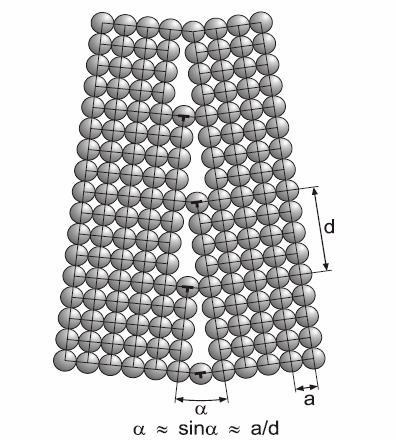
\includegraphics[width=0.5\textwidth]{Images/Korn.JPG}
	            \caption{Ätzgrübchenabstand bei Kleinwinkelkorngrenzen. [2]}
	            \label{FigKorn}
	        \end{figure}
		Die Gitterkonstante von LiF beträgt $a = 0.402$nm, der Abstand nächster Nachbarn beträgt $\frac{a}{\sqrt{2}}$. Liegen nun zwei Einkristalle in einem sehr kleinen Winkel $\alpha$ zueinander, so können wir aus dem Abstand $d$ der 
		Ätzgrübchen, die durch diese Kleinwinkelkorngrenze an der Kristalloberfläche entstehen, genau diesen Winkel bestimmen. Die Formel hierfür erhält man mithilfe
		von $\sin{\alpha} \approx \alpha$ für kleines $\alpha$ wie in Abb. \ref{FigKorn} illustriert\footnote{wobei $a$ im Bild dem Abstand nächster Nachbarn entspricht, nicht der Gitterkonstanten}:
		\begin{equation}
			\alpha \approx \frac{a}{\sqrt{2}d} = \frac{0.402nm}{\sqrt{2}d}
		\end{equation}


    \subsection{Versetzungen durch Nadeleindruck}
	\begin{figure}[H]
            \centering
            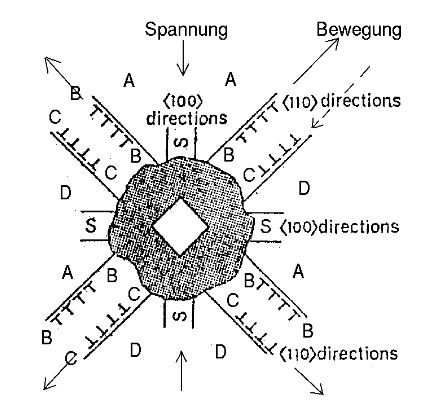
\includegraphics[width=0.6\textwidth]{Images/Question3.PNG}
            \caption{Nadeleindruck und aktivierte Gleitsysteme. [3]}
            \label{FigNadel}
        \end{figure}

	\begin{figure}[H]
            \centering
            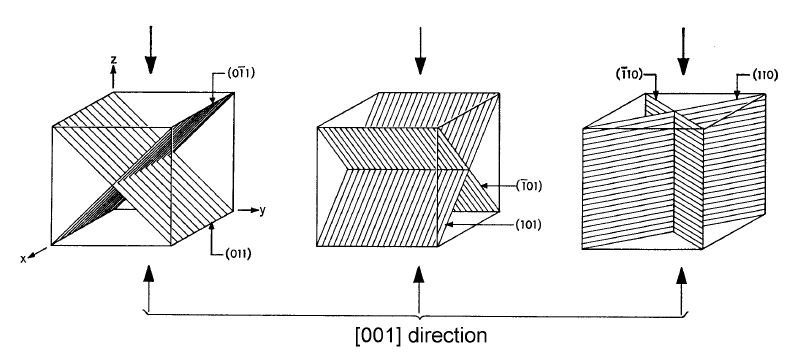
\includegraphics[width=0.7\textwidth]{Images/Gleitsysteme.JPG}
            \caption{Gleitsysteme in LiF. Quelle: Praktikumsanleitung}
            \label{FigGleitGel}
        \end{figure}
	
	Abb. \ref{FigNadel} zeigt die Rosettenform der im Versuch entstehenden Nadeleindrücke sowie die Gittervektoren, entlang derer sich die Strukturen ausbilden. 
	Die im Bild mit S gekennzeichneten Strukturen sind Schraubenversetzungen, die sich entlang der $<100>$ - Richtungen bilden. In $<110>$ - Richtung bilden sich
	Stufenversetzungen, die bei Druck auf die Probe in $\{ \overline{1}00\}$ - Richtung entlang der gekennzeichneten Richtungen wandern. Die Ursache hierfür liegt
	darin, dass bei Druck in [001] - Richtung auf die Probe jeweils die zwei Gleitsysteme von LiF aktiviert werden, die in den ersten zwei Skizzen in Abb. 
	\ref{FigGleitGel} dargestellt sind.
	


